\documentclass{}
\usepackage{tikz}
\usepackage{amsmath}
\usepackage{enumitem}
\usepackage{geometry}
\geometry{margin=1in}

\begin{document}

\section*{Sample Physics MCQ}

\textbf{Question:}  
A light ray travels from air into a glass block as shown. Which of the following best describes the behavior of the light as it enters the glass?

\begin{center}
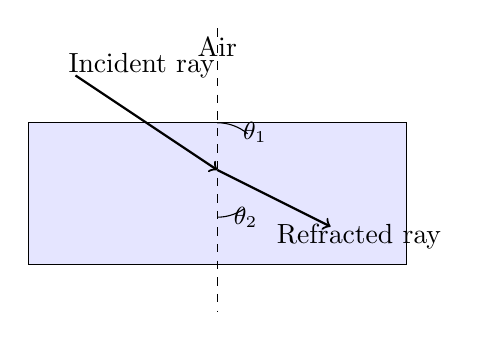
\begin{tikzpicture}[scale=1.2]
    % Air and Glass label
    \node at (2, 2.3) {Air};
    \node at (2, 0.3) {Glass};

    % Glass block
    \draw[fill=blue!10] (0,0) rectangle (4,1.5);

    % Normal line
    \draw[dashed] (2,2.5) -- (2,-0.5);

    % Incident ray
    \draw[->, thick] (0.5,2) -- (2,1);

    % Refracted ray
    \draw[->, thick] (2,1) -- (3.2,0.4);

    % Angles
    \draw (2,1) +(50:0.5) arc[start angle=50,end angle=90,radius=0.5];
    \node at (2.4,1.4) {\small $\theta_1$};

    \draw (2,1) +(270:0.5) arc[start angle=270,end angle=305,radius=0.5];
    \node at (2.3,0.5) {\small $\theta_2$};

    % Labels
    \node at (1.2,2.1) {Incident ray};
    \node at (3.5,0.3) {Refracted ray};
\end{tikzpicture}
\end{center}

\textbf{Options:}
\begin{enumerate}[label=\Alph*.]
    \item The light speeds up and bends away from the normal.  
    \item The light slows down and bends toward the normal.  
    \item The light slows down and bends away from the normal.  
    \item The light continues in a straight line.
\end{enumerate}

\vspace{1em}
\textbf{Answer:} B

\end{document}

